%%
%% This is file `tikzposter-template.tex',
%% generated with the docstrip utility.
%%
%% The original source files were:
%%
%% tikzposter.dtx  (with options: `tikzposter-template.tex')
%%
%% This is a generated file.
%%
%% Copyright (C) 2014 by Pascal Richter, Elena Botoeva, Richard Barnard, and Dirk Surmann
%%
%% This file may be distributed and/or modified under the
%% conditions of the LaTeX Project Public License, either
%% version 2.0 of this license or (at your option) any later
%% version. The latest version of this license is in:
%%
%% http://www.latex-project.org/lppl.txt
%%
%% and version 2.0 or later is part of all distributions of
%% LaTeX version 2013/12/01 or later.
%%


\documentclass{tikzposter} %Options for format can be included here

\usepackage{todonotes}

\usepackage[tikz]{bclogo}
\usepackage{lipsum}
\usepackage{amsmath}

\usepackage{booktabs}
\usepackage{longtable}
\usepackage[absolute]{textpos}
\usepackage[it]{subfigure}
\usepackage{graphicx}
\usepackage{cmbright}
%\usepackage[default]{cantarell}
%\usepackage{avant}
%\usepackage[math]{iwona}
\usepackage[math]{kurier}
\usepackage[T1]{fontenc}


%% add your packages here
\usepackage{hyperref}
% for random text
\usepackage{lipsum}
\usepackage[english]{babel}
\usepackage[pangram]{blindtext}

\colorlet{backgroundcolor}{blue!10}

 % Title, Author, Institute
\title{Sentiment Analysis on Movie Reviews}
\author{Yuhui Mou}
\institute{Xi'an Shiyou University
}
%\titlegraphic{logos/tulip-logo.eps}

%Choose Layout
\usetheme{Wave}

%\definebackgroundstyle{samplebackgroundstyle}{
%\draw[inner sep=0pt, line width=0pt, color=red, fill=backgroundcolor!30!black]
%(bottomleft) rectangle (topright);
%}
%
%\colorlet{backgroundcolor}{blue!10}

\begin{document}


\colorlet{blocktitlebgcolor}{blue!23}

 % Title block with title, author, logo, etc.
\maketitle

\begin{columns}
 % FIRST column
\column{0.5}% Width set relative to text width

%%%%%%%%%% -------------------------------------------------------------------- %%%%%%%%%%
 %\block{Main Objectives}{
%  	      	\begin{enumerate}
%  	      	\item Formalise research problem by extending \emph{outlying aspects mining}
%  	      	\item Proposed \emph{GOAM} algorithm is to solve research problem
%  	      	\item Utilise pruning strategies to reduce time complexity
%  	      	\end{enumerate}
%%  	      \end{minipage}
%}
%%%%%%%%%% -------------------------------------------------------------------- %%%%%%%%%%


%%%%%%%%%% -------------------------------------------------------------------- %%%%%%%%%%
\block{Introduction}{
    % Many real world applications call for one important function
    % of identifying the set of features
    % on which the interested object is most distinguished from others.
    % Usually,
    % this object is termed as the query object,
    % and the set of features are referred to as the \emph{subspaces} or \emph{aspects}.
    % Accordingly,
    % this research problem is referred to as
    % \emph{outlying aspects mining},
    % which is different from \emph{outlier detection}.
  	
  	% \begin{description}
  	% \item[Outlying Aspects Mining] aims to identify a subspace
    % which makes the query object most outlying,
    % rather than verifying whether it is an outlier or not.
    % The task of \emph{Outlying Aspects Mining}
    % is to explain which aspects make the query object most different.
  	
  	% \item[Outlier Detection] aims to identify all possible outliers in the dataset,
    % without explaining why or how they are different.
    % Hence,
    % the outlying aspects mining is also referred to
    % \emph{outlier interpretation}
    % or \emph{object explanation}.
  	% \end{description}

  	% In this paper,
    % we extend the task of \emph{outlying aspects mining} to the \emph{group} level,
    % formalize the research problem of \emph{group outlying aspects mining},
    % and propose a novel algorithm named GOAM to solve the
    % \emph{group outlying aspects mining} problem.
    Summary:Classify the sentiment of sentences from the Rotten Tomatoes
    dataset\\
    Every years,there are many movies appear on the screen.We can read com-
    ments to know a movie is good or not\\
    Movie Reviews come from varying people.Some may say the positive re-
    views,others may say the negative comments of the movies.We can classify
    a movie by it’s comments.But the reviews is a large dataset,people can’t read
    every comments.\\
    Here it is,we can use computer to classify the dataset.
    According to the reviews to distinguish sentiments.
}
%%%%%%%%%% -------------------------------------------------------------------- %%%%%%%%%%


%%%%%%%%%% -------------------------------------------------------------------- %%%%%%%%%%
\block{Data}{
  This event provides two data sets that can be used: train.tsv  test.tsv\\
\begin{itemize}
    \item
    %\emph{Group Outlying Aspects Mining}
    \textbf{train.tsv}: contains the phrases and their associated sentiment labels.
    We have additionally provided a SentenceId so that you can track which
    phrases belong to a single sentence.
    \item
    \textbf{test.tsv}:contains just phrases. You must assign a sentiment label to each
    phrase.
\end{itemize}

\begin{center}
    \begin{minipage}{0.3\linewidth}
    \centering
    \begin{tikzfigure}
      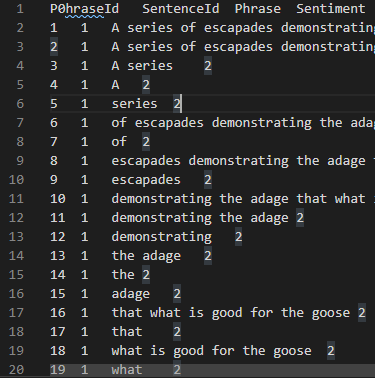
\includegraphics[width=0.9\textwidth]{D://Kaggle-test//Data//train1.png}
    {\small{train data}}
    \end{tikzfigure}%
    \end{minipage}
    \hfill
    \begin{minipage}{0.3\linewidth}
    \centering
    \begin{tikzfigure}
      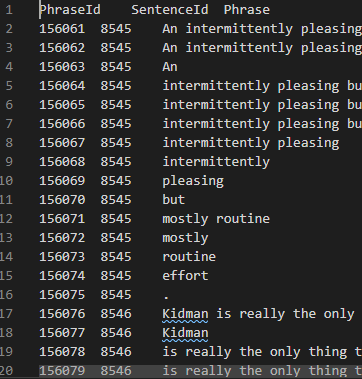
\includegraphics[width=0.9\textwidth]{D://Kaggle-test//Data//test1.png}
    {\small{test data}}
    \end{tikzfigure}%
    \end{minipage}
    \hfill 
    \begin{minipage}{0.3\linewidth}
      \centering
      \begin{tikzfigure}
        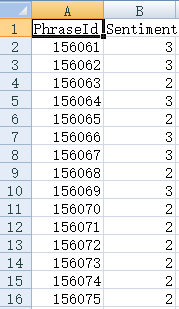
\includegraphics[width=0.9\textwidth]{D://Kaggle-test//Data//output.png}
      {\small{Group Outlying Aspects Mining}}
      \end{tikzfigure}%
      \end{minipage}
      
\end{center}
}
%%%%%%%%%% -------------------------------------------------------------------- %%%%%%%%%%


%%%%%%%%%% -------------------------------------------------------------------- %%%%%%%%%%

%\note{Note with default behavior}

%\note[targetoffsetx=12cm, targetoffsety=-1cm, angle=20, rotate=25]
%{Note \\ offset and rotated}

 % First column - second block


%%%%%%%%%% -------------------------------------------------------------------- %%%%%%%%%%
\block{Tool}{\begin{description}
  \item
  BoW\\
  The first Bag of words, also called "word bags", in information retrieval, 
  a Bag of words model assumption for a text, ignore the word order and grammar, 
  syntax, it just as a word set, or the term of a combination of, the emergence of each word in the text are independent, does not depend on whether the other word, or when the author of this article choose a word in an arbitrary position is not affected by the previous sentence and independent choice.
  The first Bag of words, also called "word bags", in information retrieval, a Bag of words model assumption for a text, ignore the word order and grammar, syntax, it just as a word set, or the term of a combination of, the emergence of each word in the text are independent, does not depend on whether the other word, or when the author of this article choose a word in an arbitrary position is not affected by the previous sentence and independent choice.
\end{description}

% \begin{tikzfigure}%[Overall architecture of \emph{GOAM} algorithm]
%     \missingfigure[figcolor=white]{Testing figcolor}
% \end{tikzfigure}
%   where $G_q$ is the query group,
%   $n$ is the number of compare groups,
%   and $h_{k_s}$ is the histogram representation of $G_k$ in the subspace $s$.

\begin{description}
\item 
TF-IDF model\\
TF - IDF (term frequency, inverse document frequency) is a kind of commonly 
used for information retrieval and data mining weighted technique, often used
 for digging the key words in the article, and the algorithm is simple and efficient,
  has often been industry for the first text data cleaning
  A word in the article the TF - the larger the IDF, so in general the word in 
  this article the importance of the higher, so each word in the article by calculation 
  of the TF - IDF, from big to small order, the top of a few words, is the key of the article
  
\end{description}
\begin{description}
  \item  Logistic Regression\\
  Used to estimate the likelihood of something, and also to classify.\\
  Logical regression is such a process: in the face of a regression or classification problem,
   the cost function is established, and then the optimal model parameters are solved iteratively through the
    optimization method, and then the quality of the model we solve is tested and verified.\\
Although Logistic regression has "regression" in its name, it is actually a classification method, 
mainly used for two classification problems (that is, there are only two outputs, representing two categories respectively).

\end{description}
% \begin{description}
%   \item 
%   RandomForestClassifier
%   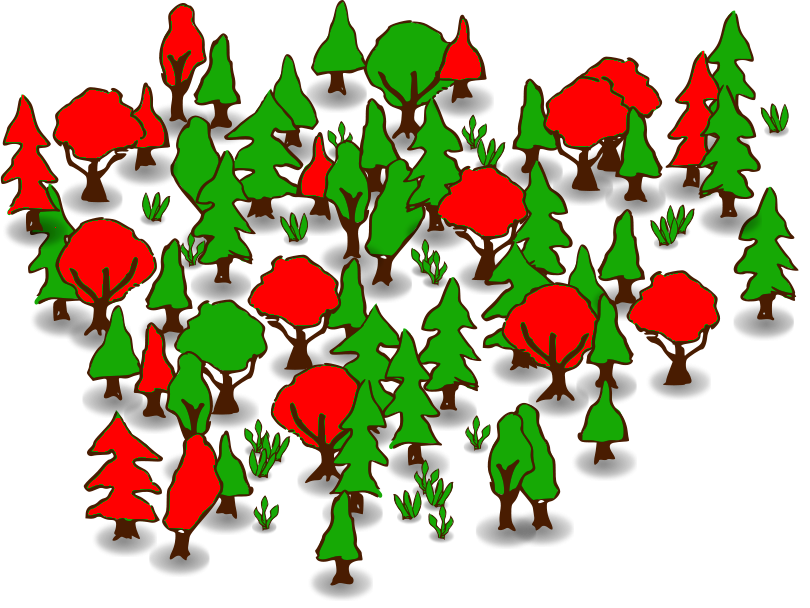
\includegraphics[width=0.2\textwidth]{D://Code//Kaggle-test//Data//suijisenlin.png}\\
%   There are many classification tree randomly in the forest. We will classify an input samples, we need to input sample input to classify each tree. Make an image of the parable: the meeting in the forest, discuss whether an animal is mouse or squirrel, every tree should be independently published his views on the question, every tree that is voting. This animal is mouse or squirrel, according to vote to determine, won the most votes category is the classification results of the forest. Each tree in the forest are independent, unrelated trees make 99.9\%  of the predicted results to cover all the situation, the forecast results will cancel each other out. A good tree prediction results will be detached from the multitude of "noise", make a good predictions. Several weak classifier classification result vote choice, so as to form a strong classifier, which is the ideas of the random forest bagging
    
% \end{description}
  
%   	We propose the \emph{GOAM} algorithm to solve the research problem of
%     \emph{Group Outlying Aspects Mining}.
%   	The \emph{GOAM} algorithm includes three major steps.
% %    1) Group Feature Extraction,
% %    2) Outlying Degree Scoring, and
% %    3) Outlying Aspects Identification.
  	
% \begin{tikzfigure}%[Overall architecture of \emph{GOAM} algorithm]
% %  \includegraphics[width=0.8\linewidth]{figures//framework.pdf}
%     \missingfigure[figcolor=white]{Testing figcolor}
% \end{tikzfigure}
		
% \begin{description}
%   	\item[Group Feature Extraction]
%   	Let $f_1$, $f_2$, $f_3$ represent three features of $G_q$.
%     We count the frequency of each value for one feature.
%     Then use the histogram to represent each feature.
%     Similarly,
%     we can extract other features for each group.

% %    \item
% %    The histogram of $G_q$ on three features are as follows.
% \end{description}

% \begin{center}
%     \begin{minipage}{0.3\linewidth}
%     \centering
%     \begin{tikzfigure}
%     \missingfigure[figcolor=white]{Testing figcolor}
%     {\small{Histogram of $G_q$ on $f_1$}}
%     \end{tikzfigure}%
%     \end{minipage}
%     \hfill
%     \begin{minipage}{0.3\linewidth}
%     \centering
%     \begin{tikzfigure}
%     \missingfigure[figcolor=white]{Testing figcolor}
%     {\small{Histogram of $G_q$ on $f_2$}}
%     \end{tikzfigure}%
%     \end{minipage}
%     \hfill
%     \begin{minipage}{0.3\linewidth}
%     \centering
%     \begin{tikzfigure}
%     \missingfigure[figcolor=white]{Testing figcolor}
%     {\small{Histogram of $G_q$ on $f_3$}}
%     \end{tikzfigure}%
%     \end{minipage}
% \end{center}
% \begin{description}
% \item[Outlying Degree Scoring]
%     In this step,
%     we first calculate the \emph{earth mover distance} (EMD) of one feature among different groups.
%     The earth mover distance reflects the minimum mean distance
%     between groups on one feature.
%     So,
%     we utilize the EMD to measure the difference between groups of each feature.
% \end{description}

}
%%%%%%%%%% -------------------------------------------------------------------- %%%%%%%%%%


% SECOND column
\column{0.5}
 %Second column with first block's top edge aligned with with previous column's top.

%%%%%%%%%% -------------------------------------------------------------------- %%%%%%%%%%
\block{Data Processing}{
  \begin{itemize}
    \item
    Read Data \\
  \begin{itemize}
  \item
  Read train.tsv
  \item
  Read test.tsv
  \end{itemize}
  \item
  Processing Model:Bag-of-words model (BoW model)\\
  \begin{itemize}
    \item 
    BoW early in Natural Language Processing and Information Retrieval 
    This model ignored the grammar and word order elements such as text, 
    just as it is a collection of several words, the emergence of each
     word in the document are independent of each otherBoW to use an 
     unordered list of words to express a text or a document.
  \end{itemize}
  \begin{itemize}
    \item 
    CountVectorizer is a characteristic class of common numerical calculation,
    Is a text feature extraction method.For each training text, it only considers 
    each of these words in the frequency of the training in the text.
    CountVectorizer Converts text of the words in the word frequency matrix.
    
  \end{itemize}
  \item 
  Logistic Regression\\
  \begin{itemize}
  \item
  The first step is using feature and target training classifier.
  \item
  The second step is to input data to classifier which has trained before.
  \item 
  Export data and Store them in a document.
  \end{itemize}

    %\emph{Group Outlying Aspects Mining}
  
\end{itemize}
}
%%%%%%%%% -------------------------------------------------------------------- %%%%%%%%%%
% Second column - first block


%%%%%%%%%% -------------------------------------------------------------------- %%%%%%%%%%
\block[titleleft]{Other Way}
{
\begin{description}
  	\item[CNN NLP] \\
  	The CNN model was initially applied in the field of image recognition. 
    Text is different from image, and pixel matrix points of image are dense, 
    but text does not have these characteristics. Each word in the sentence is represented 
    by a vector, and the vector of each word is arranged together to form a "graph", 
    which is then processed by CNN.
   
\end{description}
% \vspace{.5cm}
% \begin{tabular}{ c | c | c | c }
%     \toprule
%     Method     &  Truth Outlying Aspects    & Identified Aspects & Accuracy      \\
%     \midrule
%     GOAM       &  $\{F_1\}$, $\{F_2F_4\}$   &  $\{F_1\}$, $\{F_2F_4\}$    & 100\%    \\

%      Arithmetic Mean based OAM &  $\{F_1\}$, $\{F_2F_4\}$   &  $\{F_4\}$, $\{F_2\}$    &  0\% \\

%      Median based OAM &  $\{F_1\}$, $\{F_2F_4\}$   &  $\{F_2\}$, $\{F_4\}$    &           0\% \\
%      \bottomrule
% \end{tabular}
% \vspace{.2cm}


% \begin{description}
% \item[NBA Dataset] was collected from Yahoo Sports
% website (\url{http://sports.yahoo.com.cn/nba}).
% The data include all teams from the six divisions,
% and each player in the team has $12$ features.
% \end{description}
% \vspace{.5cm}
% \begin{tabular}{ c | c | c }
%     \toprule
%     Teams                   & Trivial Outlying Aspects  & NonTrivial Outlying Aspects    \\
%     \toprule
%     Cleveland Cavaliers     & \{3FA\}                   & \{FGA, FT\%\}, \{FGA, FG\%\} \\
%     Orlando Magic           & \{Stl\}                   & None                         \\
%     Milwaukee Bucks         & \{To\}, \{FTA\}           & \{FGA, FTA\}, \{3FA, FTA\}     \\
% %    Golden State Warriors   & \{FG\%\}                  & \{FT\%, Blk\}, \{FGA, 3PT\%, FTA\}\\
% %    Utah Jazz               & \{Blk\}                   & \{3FA, 3PT\%\}                    \\
%     New Orleans Pelicans    & \{FT\%\}, \{FTA\}         & \{FTA, Stl\}, \{FTA, To\}          \\
%     \bottomrule
% \end{tabular}
           
% 
\begin{center}
  \begin{minipage}{0.3\linewidth}
  \centering
  \begin{tikzfigure}
  \centering
    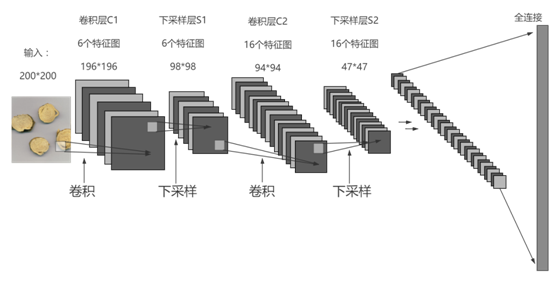
\includegraphics[width=2.0\textwidth]{D://Kaggle-test//Data//cnn.png}
  {\small{CNN}}
  \end{tikzfigure}%
  \end{minipage}
  % \hfill
  % \begin{minipage}{0.3\linewidth}
  % \centering
  % \begin{tikzfigure}
  %   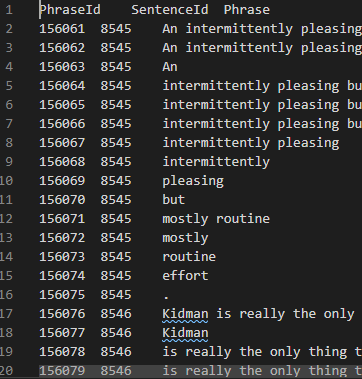
\includegraphics[width=0.9\textwidth]{D://Kaggle-test//Data//test1.png}
  % {\small{test data}}
  % \end{tikzfigure}%
  % \end{minipage}
  % \hfill 
  % \begin{minipage}{0.3\linewidth}
  %   \centering
  %   \begin{tikzfigure}
  %     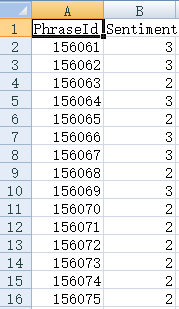
\includegraphics[width=0.9\textwidth]{D://Kaggle-test//Data//output.png}
  %   {\small{Group Outlying Aspects Mining}}
  %   \end{tikzfigure}%
  %   \end{minipage}
    
\end{center}
\begin{description}
  \item
  Before importing the text into the input layer,
You need to preprocess the text. Preprocessing includes word segmentation, depause and vectorization
It is very important to determine the word vector. When the dimension of the word vector
If it is too high, the operation times and running time of the system will be increased. When the word vector dimension is too low, it can not well reflect the word and
The approximate relationship between words and category differences affect the effect of text classification of the model. In the experiment, the accuracy of word vector 
dimension pairs is studied by testing 32, 64, 128 and 256 dimensions respectively
\end{description}
% \hfill
% \begin{minipage}{0.5\linewidth}
%     \centering
%     \begin{tikzfigure}
%     \missingfigure[figcolor=white]{Testing figcolor}

%     {\small{New Orleans Pelicans on FTA}}
%     \end{tikzfigure}%
% \end{minipage}
\vspace{.2cm}
\begin{description}
\item
The CNN model should be
For text classification, it only needs to import the preprocessed text set into the input layer, and the features will be generated automatically through model training
Words, greatly simplifies the selection of characteristic words.
% \end{description}
% \begin{description}
%   \item Humans tend to selectively block it out
%   Some unimportant information can be ignored, but pay more attention to the information considered to be important, also known as attention
%   The focal point. The attention mechanism in deep learning is essentially similar to the selective visual attention mechanism in humans, with the main purpose of
%   Devote your limited attention resources to information that is more important and critical to the task at hand.
% \end{description}
}
%%%%%%%%%% -------------------------------------------------------------------- %%%%%%%%%%


% Second column - second block
%%%%%%%%%% -------------------------------------------------------------------- %%%%%%%%%%
\block[titlewidthscale=1, bodywidthscale=1]
{Conclusion}
{
\begin{description}
  \item 
  I learned the steps of natural language processing.\\
 Know how to deal with large text class data set—-BoW model.\\
Learn a classifier-LR:can predict the test data and classify test data.\\
The CNN network model can also be used to deal with NLP problems.
\end{description}
}
%%%%%%%%%% -------------------------------------------------------------------- %%%%%%%%%%


% Bottomblock
%%%%%%%%%% -------------------------------------------------------------------- %%%%%%%%%%
\colorlet{notebgcolor}{blue!20}
\colorlet{notefrcolor}{blue!20}
\note[targetoffsetx=8cm, targetoffsety=-4cm, angle=30, rotate=15,
radius=2cm, width=.26\textwidth]{
Acknowledgement
\begin{itemize}
  \item 
  We want to thank Kaggle for providing this unique dataset. Kaggle is hosting this playground competition for fun and practice.
  The authors would like to thank \ldots
 \end{itemize}
}

%\note[targetoffsetx=8cm, targetoffsety=-10cm,rotate=0,angle=180,radius=8cm,width=.46\textwidth,innersep=.1cm]{
%Acknowledgement
%}

%\block[titlewidthscale=0.9, bodywidthscale=0.9]
%{Acknowledgement}{
%}
%%%%%%%%%% -------------------------------------------------------------------- %%%%%%%%%%

\end{columns}


%%%%%%%%%% -------------------------------------------------------------------- %%%%%%%%%%
%[titleleft, titleoffsetx=2em, titleoffsety=1em, bodyoffsetx=2em,%
%roundedcorners=10, linewidth=0mm, titlewidthscale=0.7,%
%bodywidthscale=0.9, titlecenter]

%\colorlet{noteframecolor}{blue!20}
% \colorlet{notebgcolor}{blue!20}
% \colorlet{notefrcolor}{blue!20}
% \note[targetoffsetx=-13cm, targetoffsety=-12cm,rotate=0,angle=180,radius=8cm,width=.96\textwidth,innersep=.4cm]
% {
% % \begin{minipage}{0.3\linewidth}
% % \centering
% % \includegraphics[width=24cm]{logos/tulip-wordmark.eps}
% % \end{minipage}
% \begin{minipage}{0.7\linewidth}
% { \centering
%  The $11^{th}$ International Conference on Knowledge Science,
%   Engineering and Management (KSEM 2018),
%   17-19/08/2018, Changchun, China
% }
% \end{minipage}
% }
%%%%%%%%%% -------------------------------------------------------------------- %%%%%%%%%%


\end{document}

%\endinput
%%
%% End of file `tikzposter-template.tex'.
